\documentclass{article}

\usepackage[margin=1in]{geometry}
\usepackage{amsmath,amsthm,amssymb}
\usepackage{bbm, enumerate, tikz}
\usepackage{multicol}

\newenvironment{problem}[2][Problem]{\begin{trivlist}
\item[\hskip \labelsep {\bfseries #1}\hskip \labelsep {\bfseries #2.}]}{\end{trivlist}}
\newenvironment{note}[1][Note.]{\begin{trivlist}
\item[\hskip \labelsep {\bfseries #1}]}{\end{trivlist}}

\begin{document}

\title{Spring 2012: Complex Analysis Graduate Exam}
\author{Peter Kagey}

\maketitle

% -----------------------------------------------------
% First problem
% -----------------------------------------------------
\begin{problem}{1}
  Suppose $a > 0$. Evaluate the integral \[
    \int_{-\infty}^{\infty} \frac{\sin(ax)}{x(x^2 + 1)}\, dx
  \] being careful to justify your methods.
\end{problem}

\begin{proof}
  After a transformation, this integral can be computed by using the
  \textit{Cauchy principal value} of the integral.
  In particular, the given integral can be rewritten as \[
    \int_{-\infty}^{\infty} \frac{\sin(ax)}{x(x^2 + 1)}\, dx = \int_{-\infty}^{\infty} R(x)e^{ix}\, dx
  \] where $R(x)$ is a rational function.
  First, by the substitution $u = ax$, the integral can be rewritten as
  \[
    \int_{-\infty}^{\infty} \frac{\sin(ax)}{x(x^2 + 1)}\, dx
    = \frac{1}{a} \int_{-\infty}^{\infty} \frac{\sin(u)}{\frac{u}{a}((\frac{u}{a})^2 + 1)}\, du.
    = \int_{-\infty}^{\infty} \sin(u)\frac{a^2}{u(u^2 + a^2)}\, du,
  \]
  Then by the identity $\sin(u) = -i(e^{iu} - \cos(u))$, this can be further rewritten as
  \[
    -ia^2 \int_{-\infty}^{\infty} \frac{e^{iu} - \cos(u)}{u(u^2 + a^2)}\, du
    = -ia^2 \int_{-\infty}^{\infty} \frac{e^{iu}}{u(u^2 + a^2)}\, du +
    \underbrace{
      ia^2 \int_{-\infty}^{\infty} \frac{\cos(u)}{u(u^2 + a^2)}\, du
    }_{=0\text{x, odd integrand}}
    = \int_{-\infty}^{\infty} R(u)e^{iu}\, du.
  \] where \[
    R(u) = \frac{-ia^2}{u(u^2 + a^2)}.
  \]

  Now it is enough to compute some poles and residues.
  In particular, the integrand $g(z) = R(z)e^{iz}$ has poles at $z = 0$, $z=ai$, and $z=-ai$.
  The residue $\operatorname{Res}_0(g)$ at $z=0$ can be determined from the Taylor expansion about $0$: \[
    g(z)
    = \frac{-ia^2}{z(z^2 + a^2)}e^{iz}
    = \frac{1}{z}\left(\frac{-ia^2e^{iz}}{z^2 + a^2}\right)
    = \frac{1}{z}\left[\frac{-ia^2e^{0}}{0^2 + a^2} + \hdots\right].
  \] Thus $\operatorname{Res}_0(g) = -i$.
  %
  Next, the residue $\operatorname{Res}_{ai}(g)$ can be determined similarly:
  \[
    g(z)
    = \frac{-ia^2}{z(z^2 + a^2)}e^{iz}
    = \frac{1}{z - ai}\left(\frac{-ia^2e^{iz}}{z(z + ai)}\right)
    = \frac{1}{z - ai}\left[\frac{-ia^2e^{-a}}{ai(ai + ai)} + \hdots\right].
  \]
  so $\operatorname{Res}_{ai}(g) = \frac{i}{2}e^{-a}$.
  Therefore \[
    \int_{-\infty}^{\infty} \frac{\sin(ax)}{x(x^2 + 1)}\, dx
    = 2\pi i\left[ \operatorname{Res}_{ai}(g) + \frac{1}{2}\operatorname{Res}_0(g)\right]
    = 2\pi i\left[ \frac{i}{2}e^{-a} + \frac{1}{2}(-i)\right]
    = \pi(1 - e^{-a}).
  \]
\end{proof}

% -----------------------------------------------------
% Second problem
% -----------------------------------------------------
\pagebreak

\begin{problem}{2}
  Let $f(z)$ be analytic for $0 < |z| < 1$. Assume there are $C > 0$ and
  $m \geq 1$ such that \[
    |f^{(m)}(z)| \leq \frac{C}{|z|^m},\ 0 < |z| < 1.
  \]
  Show that $f$ has a removable singularity at $z = 0$.
\end{problem}

\begin{proof}
\end{proof}

% -----------------------------------------------------
% Third problem
% -----------------------------------------------------
\pagebreak

\begin{problem}{3} Let $D \subseteq \mathbb{C}$ be a connected open subset and
  let $(u_n)$ be a sequence of harmonic functions
  $u_n\colon D \rightarrow (0, \infty)$.
  Show that if $u_n(z_0) \rightarrow 0$ for some $z_0 \in D$, then
  $u_n \rightarrow 0$ uniformly on compact subsets of $D$.
\end{problem}

\begin{proof}
\end{proof}

% -----------------------------------------------------
% Fourth problem
% -----------------------------------------------------
\pagebreak

\begin{problem}{4}
  Let $D$ be the open unit disc $\{ z \in \mathbb{C} : |z| < 1 \}$ in the
  complex plane, and define $\Omega = D \setminus [0, 1]$. Find a conformal
  mapping of $\Omega$ onto $D$. You may give your answer as the composition of
  several mappings, so long as each mapping is precisely described.
\end{problem}

\begin{proof}
  $ $ \\
  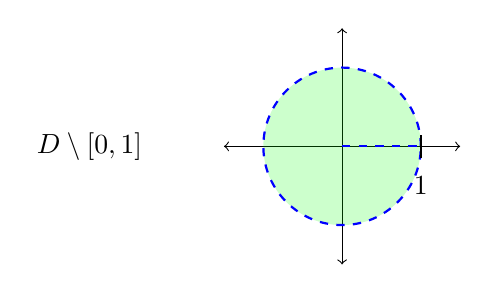
\begin{tikzpicture}
    \node[anchor=west] at (-4, 0) {$D \setminus [0, 1]$};
    \draw[<->] (-1.5,0)--(1.5,0);
    \draw[<->] (0,-1.5)--(0,1.5);
    \draw[blue, fill=green, fill opacity=0.2, thick, dashed] (0,0) circle (1);
    \draw[blue, thick, dashed] (0,0)--(1,0);
    \draw[thick] (1,-0.15)--(1,0.15);
    \node at (1,-0.5) {1};
  \end{tikzpicture}
  \hspace{0.7cm}
  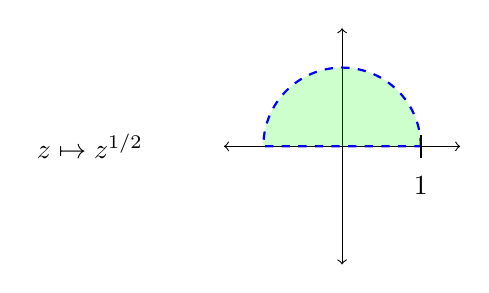
\begin{tikzpicture}
    \node[anchor=west] at (-4, 0) {$z \mapsto z^{1/2}$};
    \draw[<->] (-1.5,0)--(1.5,0);
    \draw[<->] (0,-1.5)--(0,1.5);
    \draw[blue, fill=green, fill opacity=0.2, thick, dashed] (1,0) arc (0:180:1) -- cycle;
    \draw[thick] (1,-0.15)--(1,0.15);
    \node at (1,-0.5) {1};
  \end{tikzpicture}
  \\
  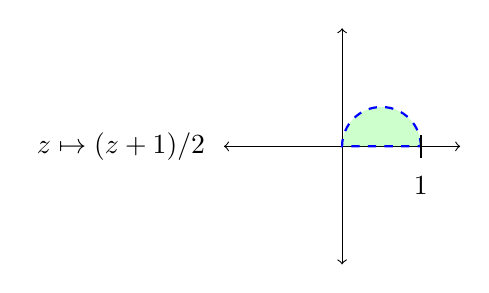
\begin{tikzpicture}
    \node[anchor=west] at (-4, 0) {$z \mapsto (z + 1)/2$};
    \draw[<->] (-1.5,0)--(1.5,0);
    \draw[<->] (0,-1.5)--(0,1.5);
    \draw[blue, fill=green, fill opacity=0.2, thick, dashed] (1,0) arc (0:180:0.5) -- cycle;
    \draw[thick] (1,-0.15)--(1,0.15);
    \node at (1,-0.5) {1};
  \end{tikzpicture}
  \hspace{0.7cm}
  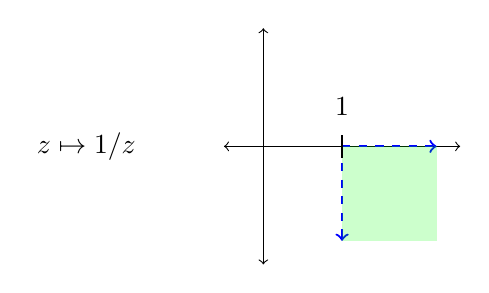
\begin{tikzpicture}
    \node[anchor=west] at (-3, 0) {$z \mapsto 1/z$};
    \draw[<->] (-0.5,0)--(2.5,0);
    \draw[<->] (0,-1.5)--(0,1.5);
    \draw[thick, dashed, blue, ->] (1,0)--(2.2,0);
    \draw[thick, dashed, blue, ->] (1,0)--(1,-1.2);
    % \draw[blue, fill=green, fill opacity=0.2, thick, dashed] (1,0) arc (0:180:0.5) -- cycle;
    \fill[green, opacity=0.2] (1,0) rectangle (2.2,-1.2);
    \draw[thick] (1,-0.15)--(1,0.15);
    \node at (1,0.5) {1};
  \end{tikzpicture}
  \\
  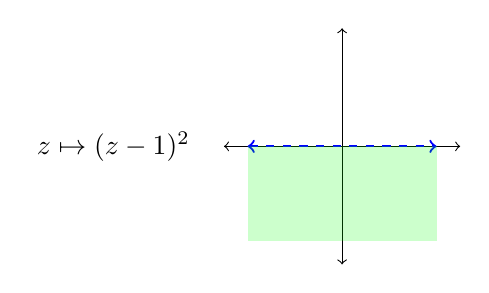
\begin{tikzpicture}
    \node[anchor=west] at (-4, 0) {$z \mapsto (z - 1)^2$};
    \draw[<->] (-1.5,0)--(1.5,0);
    \draw[<->] (0,-1.5)--(0,1.5);
    \draw[thick, dashed, blue, <->] (-1.2,0)--(1.2,0);
    \fill[green, opacity=0.2] (-1.2,0) rectangle (1.2,-1.2);
  \end{tikzpicture}
  \hspace{0.7cm}
  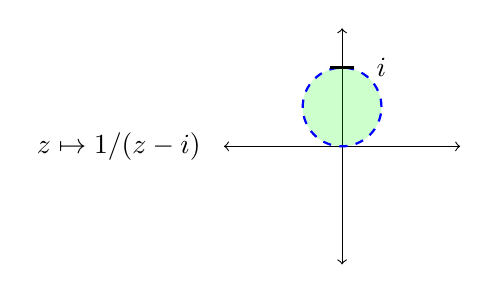
\begin{tikzpicture}
    \node[anchor=west] at (-4, 0) {$z \mapsto 1/(z - i)$};
    \draw[<->] (-1.5,0)--(1.5,0);
    \draw[<->] (0,-1.5)--(0,1.5);
    % \draw[]
    \draw[thick, dashed, blue, fill=green, fill opacity=0.2] (0,0.5) circle (0.5);
    % \fill[green, opacity=0.2] (-1.2,0) rectangle (1.2,-1.2);
    \draw[thick] (-0.15,1)--(0.15,1);
    \node at (0.5, 1) {$i$};
  \end{tikzpicture}
  \\
  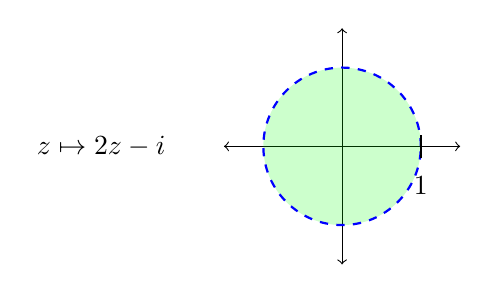
\begin{tikzpicture}
    \node[anchor=west] at (-4, 0) {$z \mapsto 2z - i$};
    \draw[<->] (-1.5,0)--(1.5,0);
    \draw[<->] (0,-1.5)--(0,1.5);
    \draw[blue, fill=green, fill opacity=0.2, thick, dashed] (0,0) circle (1);
    % \draw[blue, thick, dashed] (0,0)--(1,0);
    \draw[thick] (1,-0.15)--(1,0.15);
    \node at (1,-0.5) {1};
  \end{tikzpicture}
\end{proof}

\end{document}
